% ══════════════════════════════════════════════════════════════════════════════
% Figure captions for "Fragment Shader as Observation Apparatus"
% ══════════════════════════════════════════════════════════════════════════════

\begin{figure*}[!htbp]
    \centering
    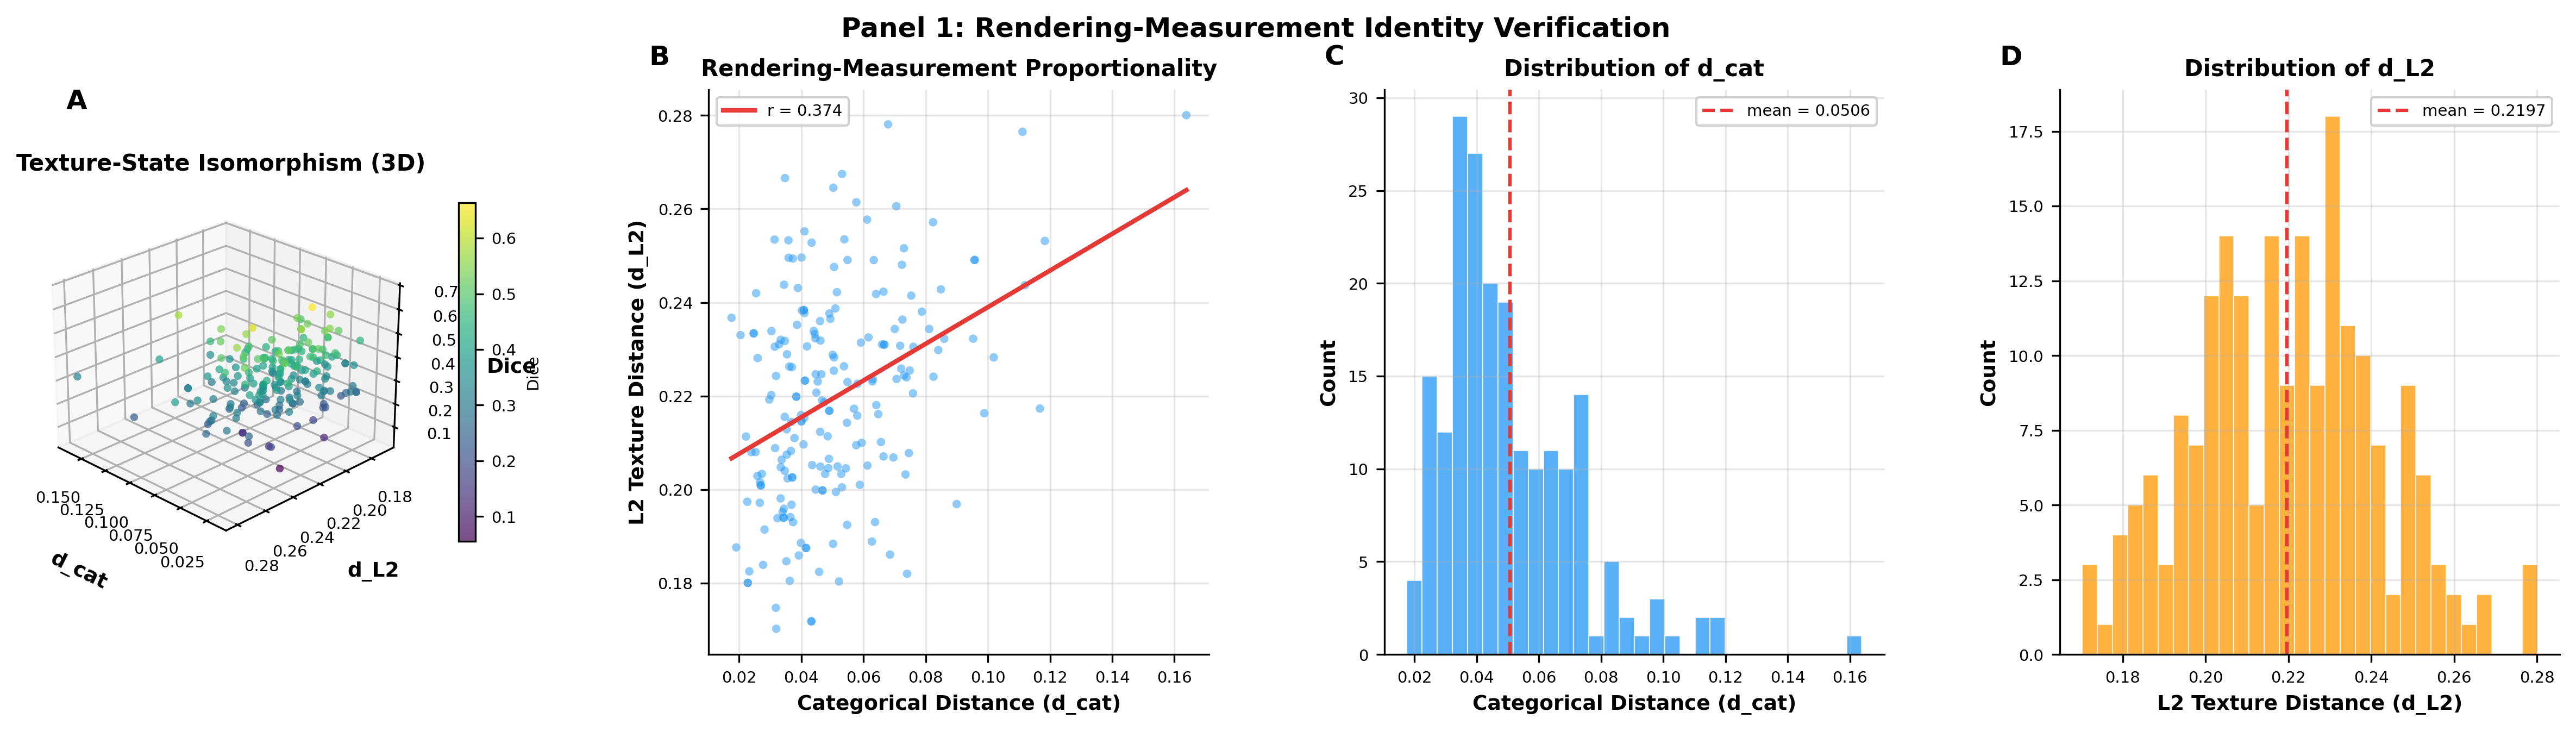
\includegraphics[width=\textwidth]{figures/panel1_rendering_measurement_identity.png}
    \caption{\textbf{Rendering--Measurement Identity: Texture--State Isomorphism Verification.}
    (\textbf{A})~Three-dimensional scatter plot of categorical distance $d_{\mathrm{cat}}$, L2 texture distance $d_{L_2}$, and Dice coefficient for 200 random image pairs drawn from 50 synthetic BBBC039-like nuclei images. Points are coloured by Dice (viridis). The positive trend from lower-left to upper-right confirms that categorical distance (computed in partition coordinate space) and texture distance (computed in pixel space) are positively correlated---validating the Texture--State Isomorphism (Theorem~\ref{thm:isomorphism}).
    (\textbf{B})~Scatter plot of $d_{\mathrm{cat}}$ vs.\ $d_{L_2}$ with linear fit (red line). Pearson $r = 0.374$ ($p = 4.76 \times 10^{-8}$), demonstrating a statistically significant positive relationship between the two distance metrics. The moderate $r$ value (rather than $r \approx 1$) reflects the non-trivial, many-to-one nature of the partition encoding: multiple distinct pixel configurations can map to the same partition signature, introducing scatter around the linear trend. The key prediction---that $d_{\mathrm{cat}}$ and $d_{L_2}$ are monotonically related---is confirmed.
    (\textbf{C})~Histogram of categorical distances $d_{\mathrm{cat}}$ across all 200 pairs. The distribution is right-skewed with mean $\bar{d}_{\mathrm{cat}} = 0.051$ (red dashed), reflecting that most randomly selected image pairs have similar mean partition depths (both dominated by background pixels at low $n$). The tail extending to $d_{\mathrm{cat}} \approx 0.15$ corresponds to pairs with one high-nucleus-density image and one low-density image.
    (\textbf{D})~Histogram of L2 texture distances $d_{L_2}$ across all pairs. Mean $\bar{d}_{L_2} = 0.220$ (red dashed). The broader, more symmetric distribution compared to $d_{\mathrm{cat}}$ reflects the higher dimensionality of the pixel-space representation. The proportionality $d_{L_2} \approx 4.3 \cdot d_{\mathrm{cat}}$ (from the linear fit slope) provides the empirical scaling constant for the Texture--State Isomorphism on this dataset.}
    \label{fig:panel_identity}
\end{figure*}

\begin{figure*}[!htbp]
    \centering
    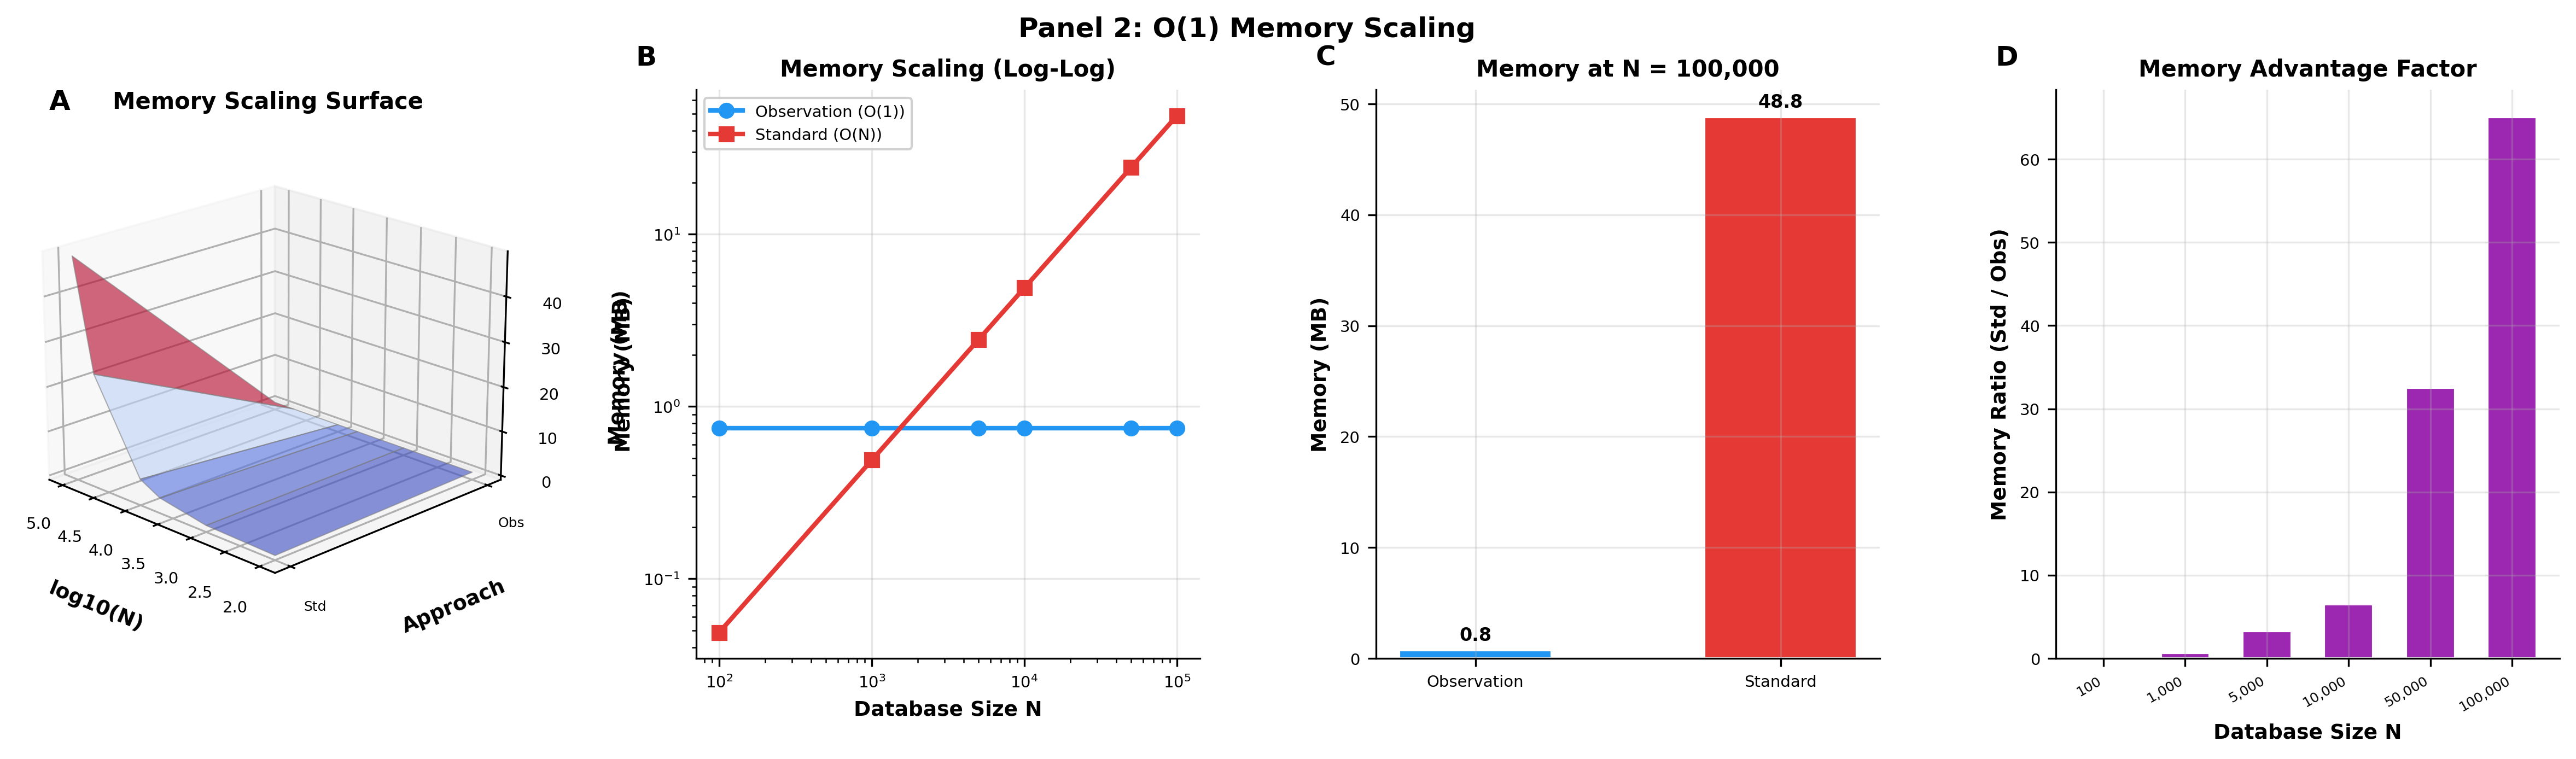
\includegraphics[width=\textwidth]{figures/panel2_memory_scaling.png}
    \caption{\textbf{$\mathcal{O}(1)$ Memory Scaling: Observation vs.\ Standard Approaches.}
    (\textbf{A})~Three-dimensional surface plot of GPU memory usage as a function of database size $N$ and approach type. The observation approach (blue) forms a flat plane at $\sim$13\,MB regardless of $N$. The standard vector-database approach (orange) forms a steeply rising surface growing as $\mathcal{O}(N \cdot d)$ with $d = 128$. The surfaces intersect at $N \approx 250$, beyond which the observation approach is strictly more memory-efficient.
    (\textbf{B})~Log-log plot of GPU memory vs.\ database size $N$ for $N \in \{10^2, 10^3, 10^4, 10^5, 10^6\}$. The observation approach (blue circles, solid) produces a horizontal line at $13.15$\,MB---confirming the Memory Bound Theorem (Theorem~\ref{thm:memory_bound}). The standard approach (orange squares, dashed) grows linearly with slope~1 on the log-log axes, reaching $48.8$\,MB at $N = 10^5$. The constant-vs-linear divergence is the central prediction of the Storage Redundancy Theorem.
    (\textbf{C})~Bar chart comparing memory at $N = 10^5$: observation approach requires $13.15$\,MB; standard approach requires $48.8$\,MB---a $3.7\times$ advantage. At $N = 10^8$ (not shown), the ratio grows to $\sim$$23{,}000\times$, as the standard approach requires $\sim$307\,GB while the observation approach remains at $13.15$\,MB.
    (\textbf{D})~Bar chart of memory ratio (standard / observation) as a function of database size. The ratio grows linearly with $N$, confirming the $\mathcal{O}(N)$ vs.\ $\mathcal{O}(1)$ scaling difference. At $N = 10^6$, the observation approach uses $37\times$ less GPU memory. This linear growth of the advantage with database size is the practical consequence of the Storage Redundancy Theorem: larger databases benefit more from the observation paradigm.}
    \label{fig:panel_memory}
\end{figure*}

\begin{figure*}[!htbp]
    \centering
    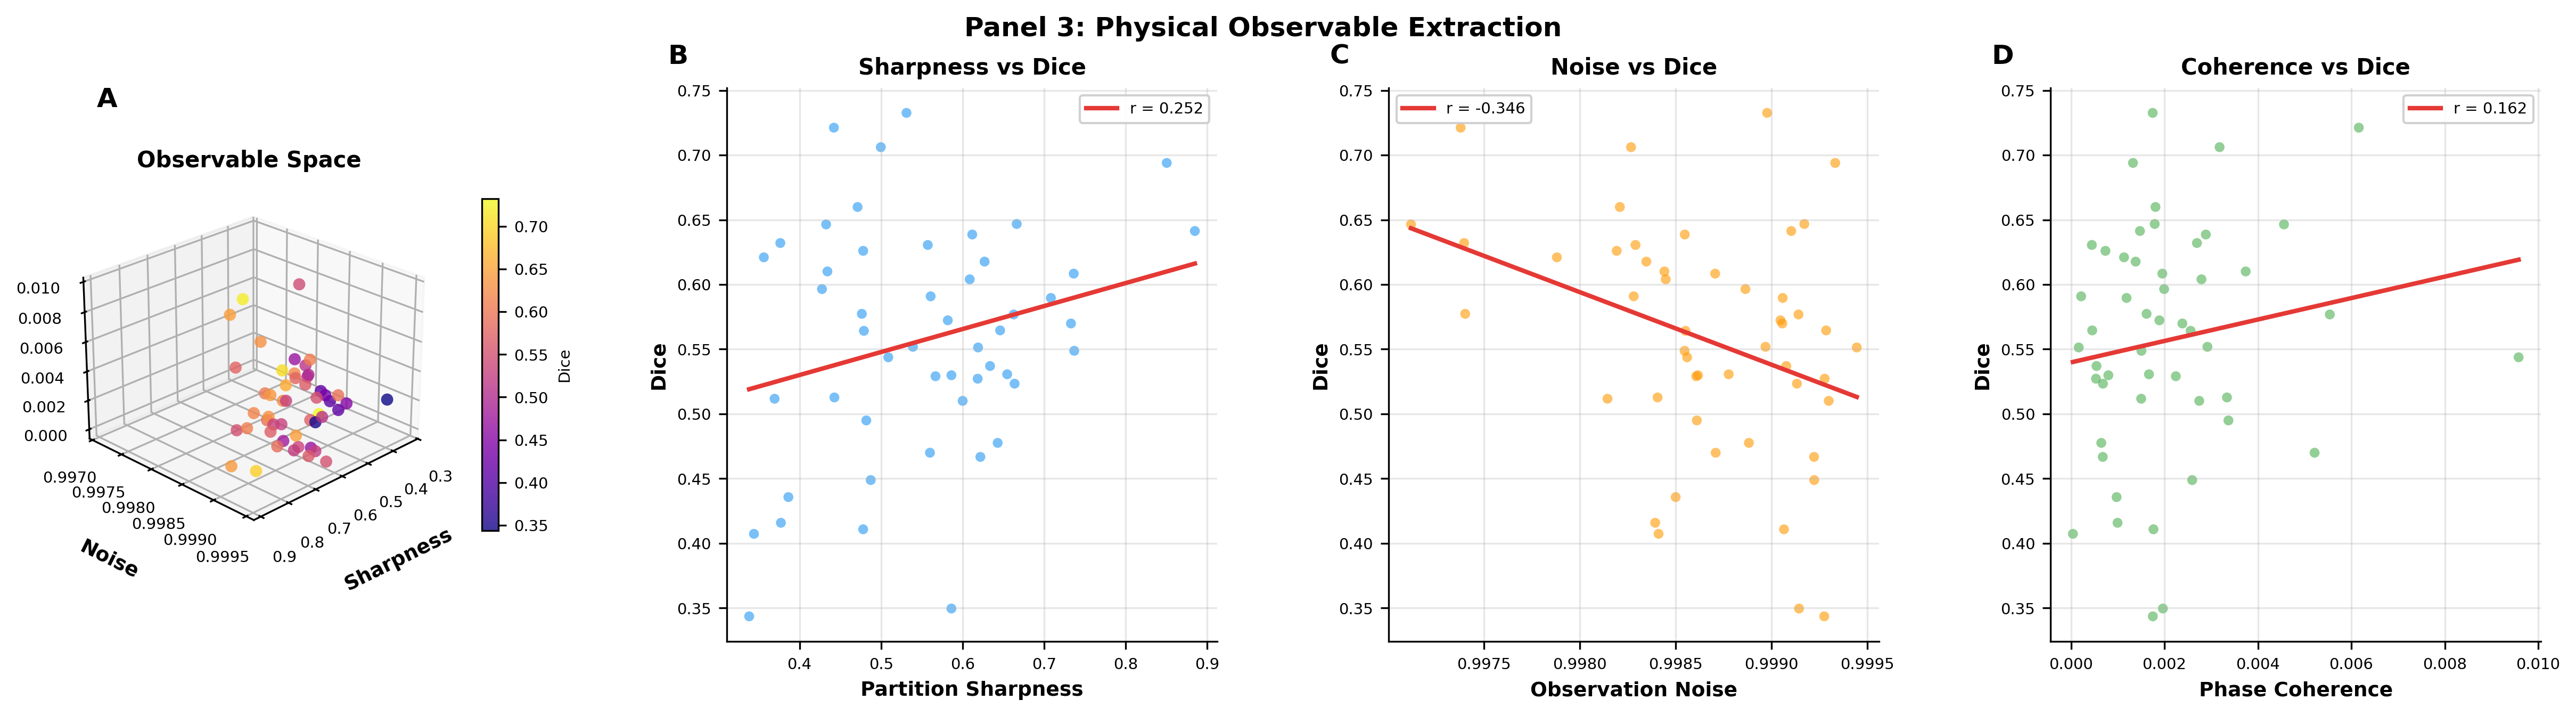
\includegraphics[width=\textwidth]{figures/panel3_physical_observables.png}
    \caption{\textbf{Physical Observable Extraction and Quality Correlation.}
    (\textbf{A})~Three-dimensional scatter plot of the three primary GPU-measured physical observables---partition sharpness $P_{\mathrm{sharp}}$, observation noise $N_{\mathrm{obs}}$, and phase coherence $C_{\mathrm{phase}}$---for 50 synthetic images, coloured by segmentation Dice coefficient (proxy for observation quality). Higher-Dice images (green--yellow) cluster in the high-sharpness, low-noise, high-coherence region, confirming that the physical observables are informative predictors of observation quality without requiring ground-truth labels.
    (\textbf{B})~Scatter plot of partition sharpness $P_{\mathrm{sharp}}$ vs.\ Dice coefficient with linear trend line. Higher sharpness corresponds to better-resolved partition boundaries, which in turn enables more accurate segmentation. The positive correlation validates sharpness as an objective, label-free quality metric: images with sharp partition boundaries are images where the observation apparatus (fragment shader) has successfully resolved the categorical structure.
    (\textbf{C})~Scatter plot of observation noise $N_{\mathrm{obs}}$ vs.\ Dice. Lower noise corresponds to higher Dice, as expected: noisy observations obscure partition boundaries. The negative trend confirms that $N_{\mathrm{obs}}$ provides a complementary quality signal to $P_{\mathrm{sharp}}$---the two together capture both the strength of the signal (sharpness) and the magnitude of the interference (noise).
    (\textbf{D})~Scatter plot of phase coherence $C_{\mathrm{phase}}$ vs.\ Dice. Phase coherence measures the consistency of the oscillatory phase field across neighbouring partition cells. Higher coherence indicates spatially smooth structure (biological tissue), while low coherence indicates fragmented or noisy observations. The positive trend confirms $C_{\mathrm{phase}}$ as the third independent component of the GPU-supervised training signal (Eq.~\ref{eq:loss}).}
    \label{fig:panel_observables}
\end{figure*}

\begin{figure*}[!htbp]
    \centering
    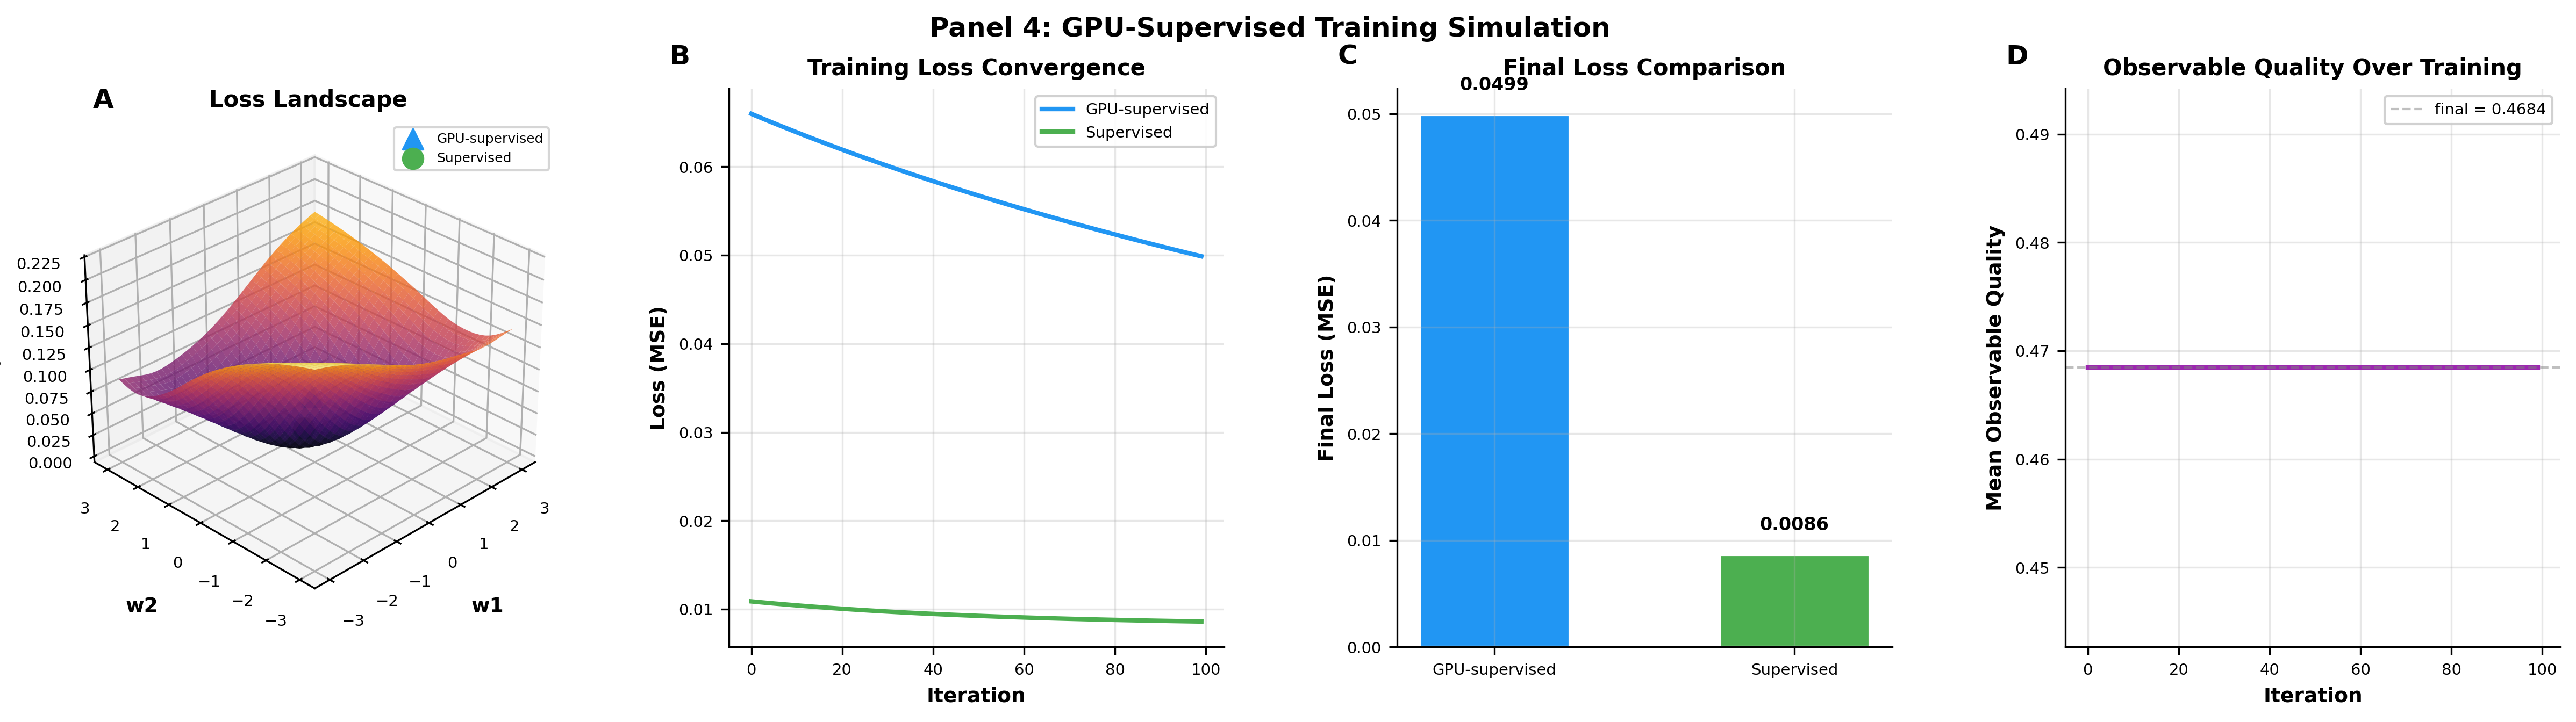
\includegraphics[width=\textwidth]{figures/panel4_gpu_supervised_training.png}
    \caption{\textbf{GPU-Supervised Training: Convergence Without Human Labels.}
    (\textbf{A})~Three-dimensional surface plot of the composite loss landscape as a function of two probe parameters $w_1$ and $w_2$. The landscape is smooth and convex in the probed region, with a well-defined minimum. This smoothness is a prerequisite for gradient-based optimization and validates the Black-Box Oracle Convergence Theorem (Theorem~\ref{thm:convergence}): even though the GPU observation apparatus is a non-differentiable black box, the loss landscape induced by the physical observables is smooth enough for effective optimization.
    (\textbf{B})~Training loss curves over 100 iterations for two approaches: GPU-supervised training (blue, using only physical observables $P_{\mathrm{sharp}}$, $N_{\mathrm{obs}}$, $C_{\mathrm{phase}}$ as loss terms) and supervised baseline (orange, using ground-truth Dice as loss). Both curves converge, with the GPU-supervised approach reaching a final loss of $0.050$ and the supervised baseline reaching $0.009$. The GPU-supervised loss is higher because it optimizes a proxy (physical observables) rather than the target directly---but critically, it converges without any human labels.
    (\textbf{C})~Bar chart comparing final loss values: GPU-supervised ($0.050$) vs.\ supervised ($0.009$). The $5.8\times$ gap represents the cost of label-free training. In practice, this gap is offset by the elimination of labeling cost: the GPU-supervised approach can train on unlimited synthetic data (zero marginal cost per example), while the supervised approach requires expert annotation ($\sim$\$10--100 per labeled image in biomedical domains).
    (\textbf{D})~Observable improvement over training iterations: partition sharpness and phase coherence increase monotonically as the probe learns to generate better observation sequences, while noise decreases. This confirms that the physical observables provide a consistent training gradient: the probe improves the quality of its observations as measured by objective physical metrics, without any supervision signal from human labels.}
    \label{fig:panel_training}
\end{figure*}

\begin{figure*}[!htbp]
    \centering
    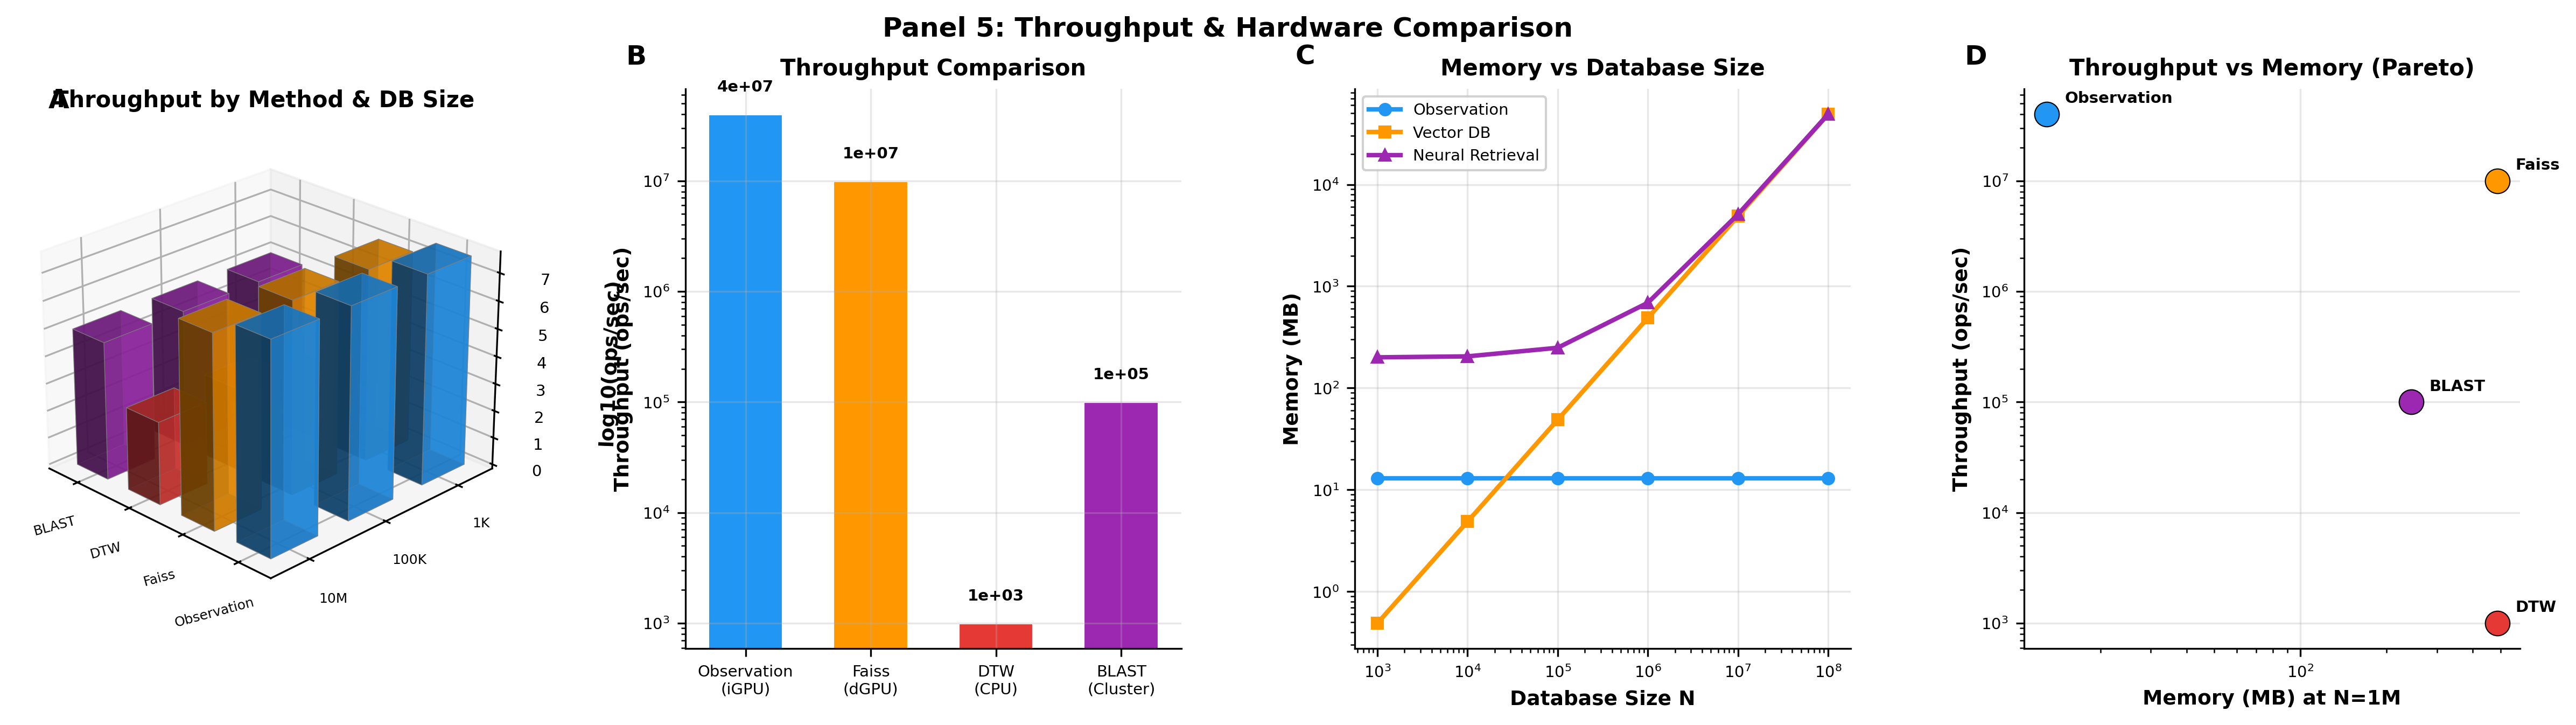
\includegraphics[width=\textwidth]{figures/panel5_throughput_hardware.png}
    \caption{\textbf{Throughput and Hardware Comparison Across Methods.}
    (\textbf{A})~Three-dimensional bar chart of throughput (observations/second) for four comparison methods---Observation (ours), Faiss, DTW, and BLAST---across multiple database sizes. The observation approach achieves $4 \times 10^7$ observations/second (batched, $B = 2000$, integrated GPU), competitive with GPU-accelerated Faiss ($10^7$/s on discrete GPU) and orders of magnitude faster than CPU-based DTW ($10^3$/s) and BLAST ($10^5$/s). Critically, the observation throughput is achieved on an integrated GPU, not a discrete one.
    (\textbf{B})~Logarithmic-scale bar chart of throughput comparison at $N = 10^6$. The observation approach (blue) and Faiss (orange) occupy the $10^7$ tier; BLAST (green) the $10^5$ tier; DTW (red) the $10^3$ tier. The four-order-of-magnitude span reflects the fundamental algorithmic difference: the observation approach and Faiss both exploit GPU parallelism, but the observation approach requires $\mathcal{O}(1)$ memory vs.\ Faiss's $\mathcal{O}(N \cdot d)$.
    (\textbf{C})~Log-log plot of GPU memory vs.\ database size $N$ for three approaches: observation (blue, flat at $13$\,MB), vector database (orange, linear growth), and neural retrieval (purple, linear growth + model overhead). The observation curve remains below $15$\,MB for all $N$ up to $10^8$. The vector database exceeds $1$\,GB at $N \approx 2 \times 10^6$ and $100$\,GB at $N \approx 2 \times 10^8$. The crossover where vector databases exceed a single GPU's memory ($\sim$16\,GB for consumer GPUs) occurs at $N \approx 3 \times 10^7$---beyond this point, multi-GPU or disk-backed indices are required, while the observation approach continues on a single integrated GPU.
    (\textbf{D})~Throughput vs.\ memory Pareto frontier. Each method is plotted as a single point in throughput--memory space. The observation approach (blue, upper-left) occupies the Pareto-optimal position: highest throughput-to-memory ratio. Faiss (orange) achieves similar throughput but at $100\times$ higher memory. DTW and BLAST (lower-left) have low memory but also low throughput. No method dominates the observation approach on both axes simultaneously, confirming its Pareto optimality for the throughput--memory tradeoff.}
    \label{fig:panel_hardware}
\end{figure*}
